\documentclass[tikz,border=3.14mm]{standalone}
\usepackage{amsmath}
\usetikzlibrary{intersections,calc}

\begin{document}
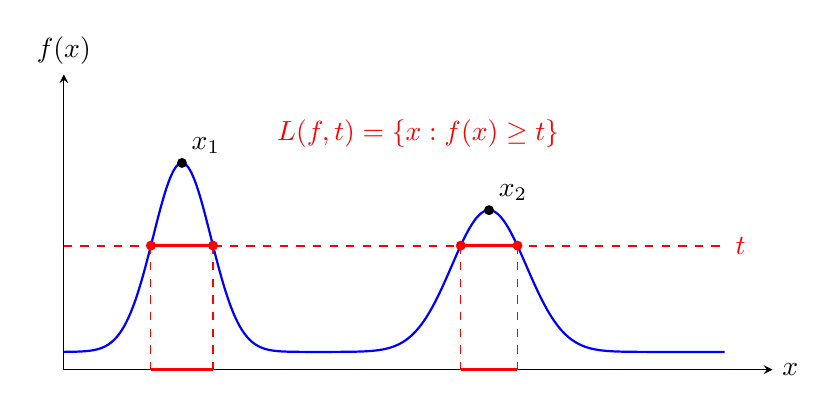
\begin{tikzpicture}[>=stealth, scale=1.5]

% 坐标轴
\draw[->] (0,0) -- (6,0) node[right] {$x$};
\draw[->] (0,0) -- (0,2.5) node[above] {$f(x)$};

% 函数表达式(两个高斯峰)
\newcommand{\f}[1]{0.15 + 1.6*exp(-((#1-1.0)^2)/0.12) + 1.2*exp(-((#1-3.6)^2)/0.20)}

% 函数路径, 命名为 fpath
\path[name path=fpath] plot[variable=\x, domain=0:5.6, samples=400] 
    ({\x}, {\f{\x}});
\draw[thick, blue, smooth] plot[variable=\x, domain=0:5.6, samples=400] 
    ({\x}, {\f{\x}});

% 水平线 t(取在两峰间低谷之上, 确保有 4 个交点)
\def\t{1.05}
\path[name path=hline] (0,\t) -- (5.6,\t);
\draw[red, thick, dashed] (0,\t) -- (5.6,\t) node[right] {$t$};

% 明确求出四个交点 P1..P4(若确实存在)
\path[name intersections={of=fpath and hline, by={P1,P2,P3,P4}}];

% 画交点并垂直投影到 x 轴
\foreach \i in {1,2,3,4} {
  \fill[red] (P\i) circle (1.2pt);
  \draw[red, dashed] (P\i) -- (P\i |- 0,0);
  \node[below] at (P\i |- 0,0) {\small $\,$}; % 占位以保持对齐
}

% 在水平线上突出上水平集区间, 并在 x 轴上显示投影区间
\draw[red, very thick] (P1) -- (P2); % 在水平线上突出第一段
\draw[red, very thick] (P3) -- (P4); % 在水平线上突出第二段
\draw[red, very thick] (P1 |- 0,0) -- (P2 |- 0,0); % x 轴投影段 1
\draw[red, very thick] (P3 |- 0,0) -- (P4 |- 0,0); % x 轴投影段 2

% 给交点在 x 轴上标记 a,b,c,d
% \node[below] at (P1 |- 0,0) {$a$};
% \node[below] at (P2 |- 0,0) {$b$};
% \node[below] at (P3 |- 0,0) {$c$};
% \node[below] at (P4 |- 0,0) {$d$};

% 标注上水平集
\node[red] at (3.0,2.0) { $L(f,t)=\{x: f(x)\ge t\}$};

% 峰点标记
\fill[black] (1.00, {\f{1.00}}) circle (1.2pt) node[above right] {$x_1$};
\fill[black] (3.60, {\f{3.60}}) circle (1.2pt) node[above right] {$x_2$};

% 说明文字
% \node[align=left] at (3.0,0.35) {
%   \small 上水平集为闭区间并:$L(f,t)=[a,b]\cup[c,d]$。
% };

\end{tikzpicture}
\end{document}
